
\chapter{Solid Rotor Technology}
\label{chap:Solid-Rotor-Technology}

% ---------------------------------------------------------------------------------------------

In industrial settings, the Polyphase induction motors (IMs) have shown clear advantages due
their efficiency and construction simplicity as over more than a century of work and research
went into improving its overall performance. These structural optimization along with the
industries lack of need for constant torque output in the industry made IMs the preferred
choice.  Furthermore their most distinctive characteristic is, by using different types of
rotor construction, different types of torque characteristics can be achieved.

The most common type of IM is the Squirrel-Cage IM (CRIM). Such a motor consists of a steel
cylinder, with the slots being filled with mostly aluminum conductors. The rotor structure is
laminated to decrease the eddy currents that are being induced in the rotor. These currents are
the main cause of eddy current losses in a rotor. The skewed body structure also helps the
rotor to avoid the cogging torque at its start of operation. The skewed design also indirectly
help in the increase of the total rotor impendence, which in turn increase the starting torque.

% Figure 2.1

Although a cage-induction machine has widespread use in industrial applications, the weakness
of its structure for high-speed implementation limits its use to the current range of
applications. Depending on the structural complexity, the rotor design has several constraints
that limit its operation in terms of angular speed, since the rotor cannot withstand the large
rotational stresses caused by the high circumferential velocity of the rotor. Practical studies
have shown that a squirrel- cage rotor cannot operate at speeds of 50,000 rpm [1].

Even though squirrel-cage IM is not possible to use in high-speed application various
alternatives have been proposed. One of the most promising one is to use a solid body equipped
with a squirrel cage [22,23,24]. A solid body with a squirrel cage is made from a ferromagnetic
material such as Fe52 (S355J0/EN 10025), while the squirell cage is made from copper
alloy. Howeveri the construction of this type of rotor is complicated and with the presence of
various parts it is not a popular choice in high-speed applications.

\begin{figure}[t]
  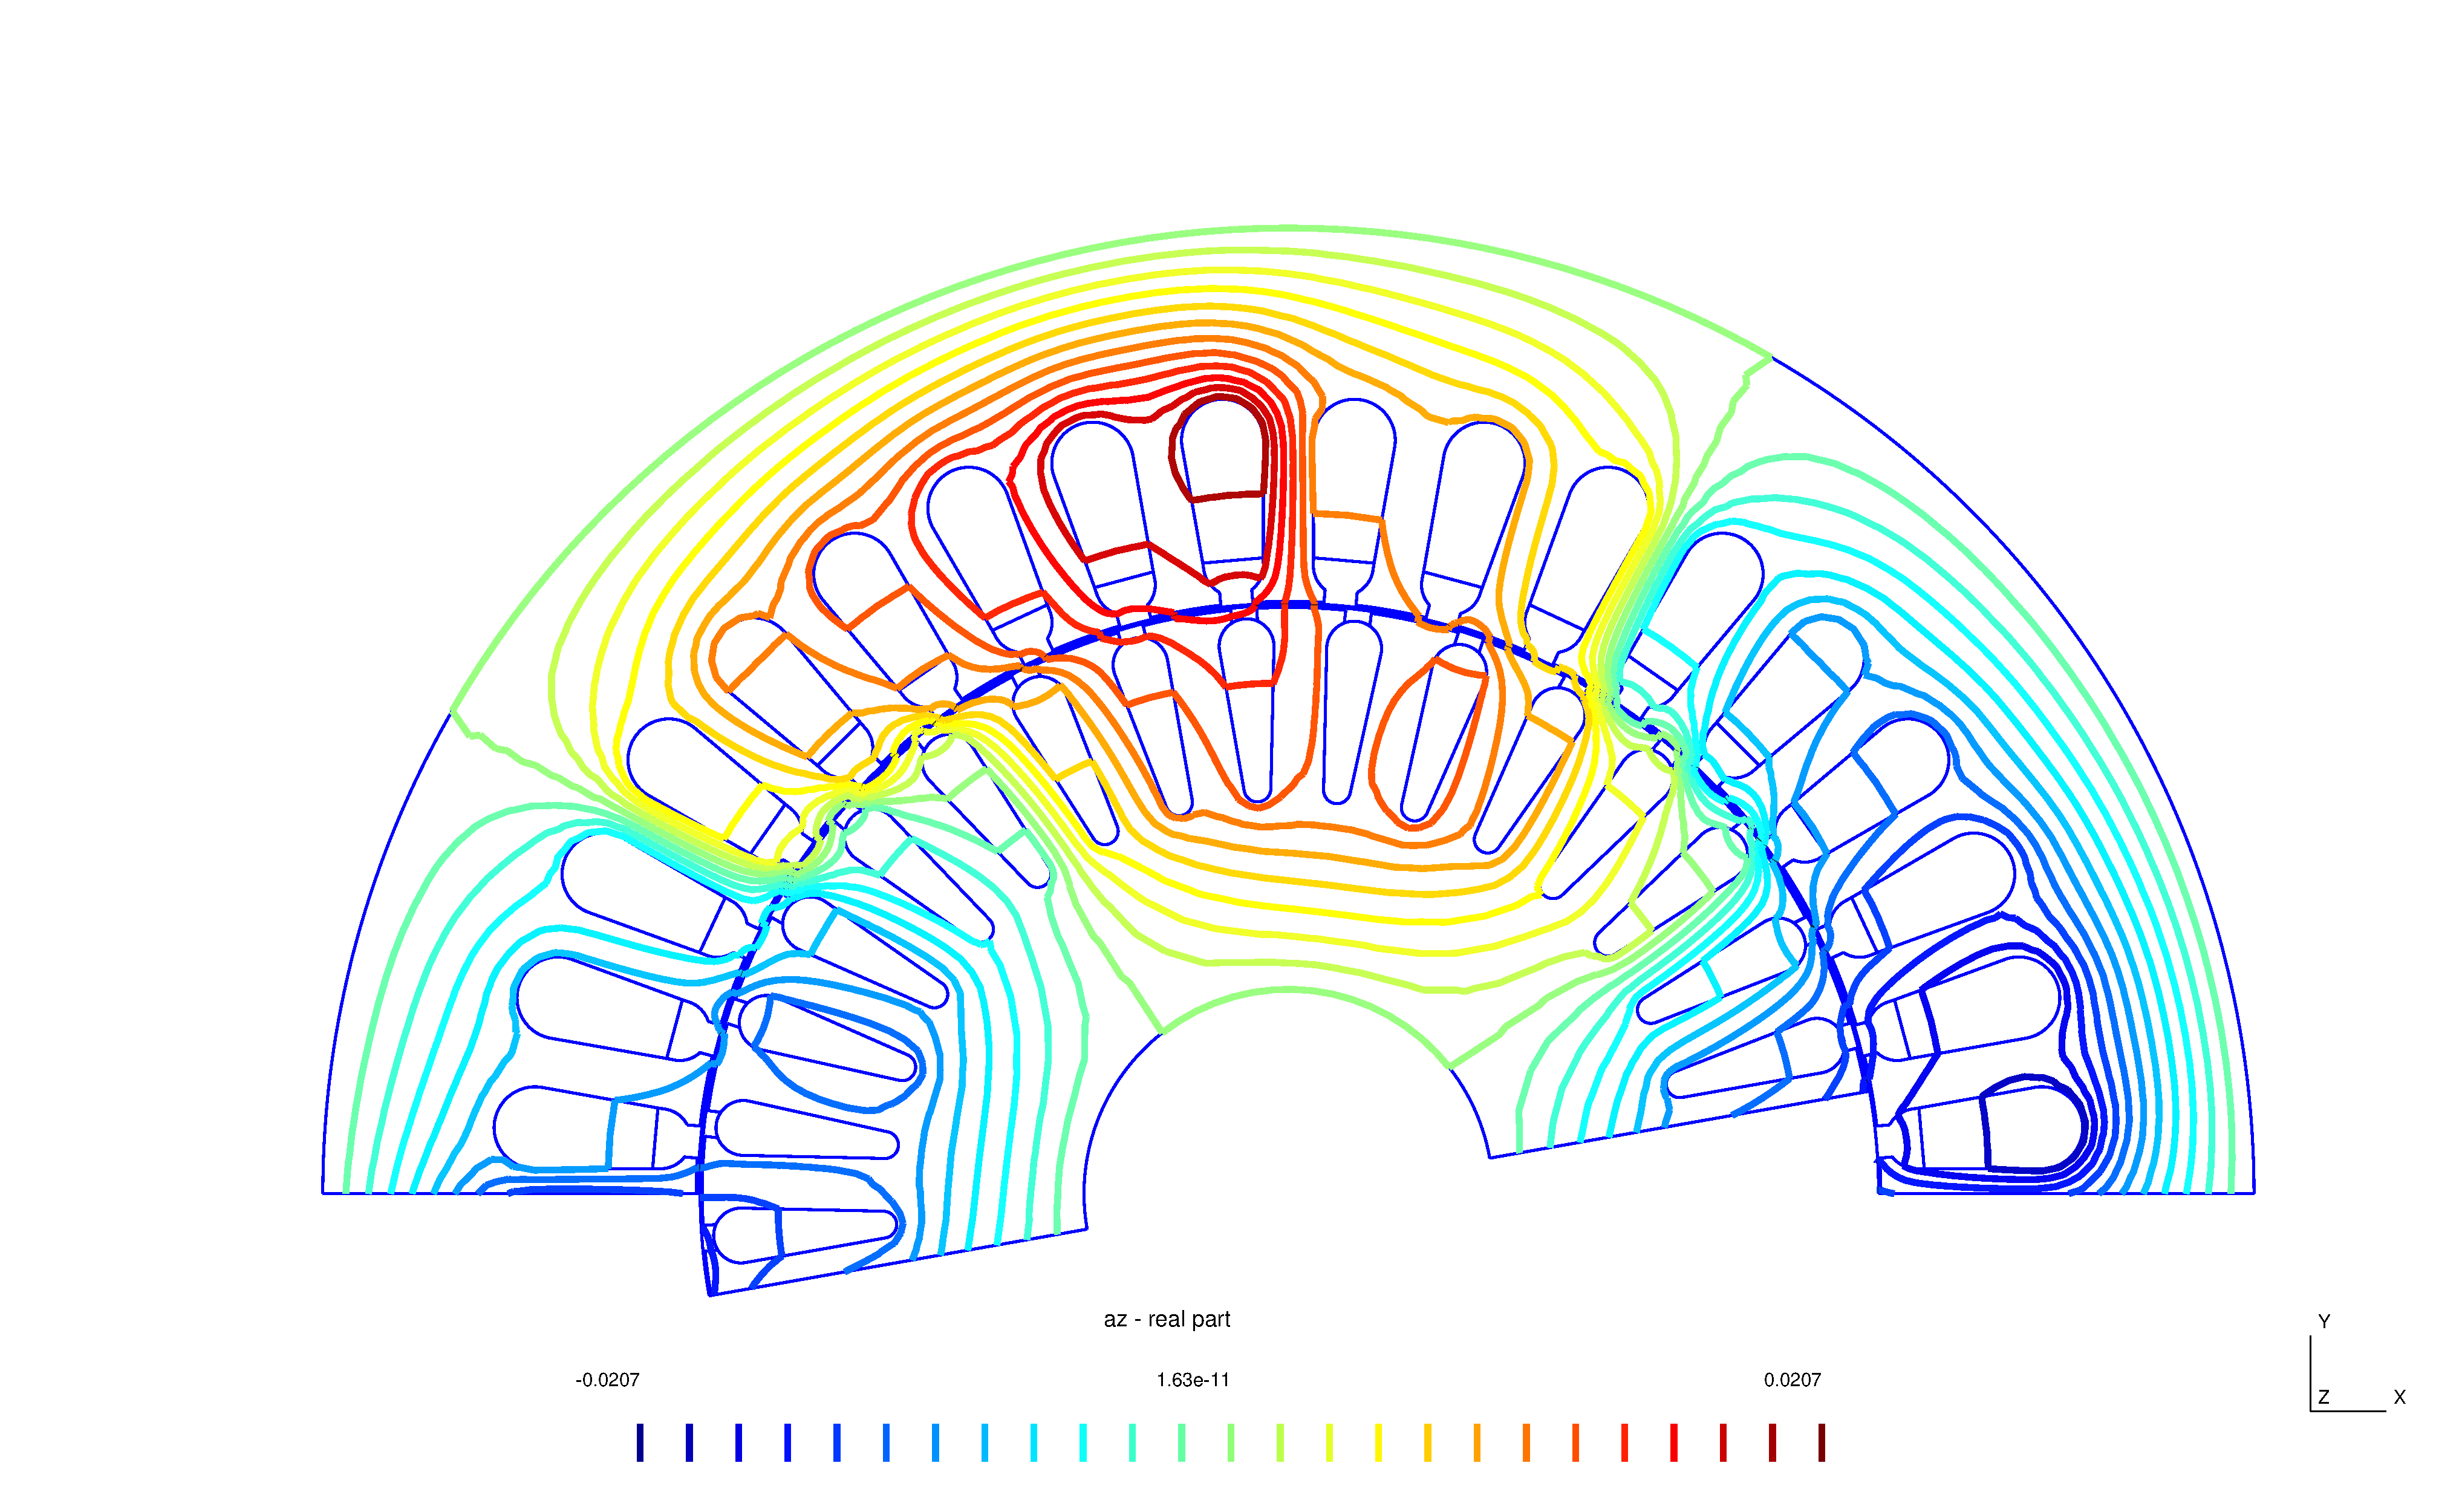
\includegraphics[width=\textwidth]{figures/im_3kW.pdf}
\end{figure}

\section{Introduction} %#######################################################################

When a high-speed application is targeted, a solid rotor is by far the better choice.
The motors with solid rotors have advantages over other types of induction motor in
terms of mechanical strength and structural simplicity, as well as being easier to
manufacture [25]. Solid-rotor Induction Motor is built from a rotor made of a single
piece of ferromagnetic material. For this reason, solid rotors are superior to
conventional cage-rotor structures in terms of their ability to operate in extremely
high-speed applications and their durability with respect to high thermal stresses that
ensure low levels of vibrations under all operating conditions [20].

As it is known the construction of a CRIM requires complex production methods.
By developing solid rotors we can overcome the complexity of IM manufacturing.
Apart from the advantages of the SRIM mentioned above, the others are given
below. These are mainly;
\begin{itemize}
\item If the rotor is a SSRIM motor, because of the absence of slots there will be no vibrations or noise
\item  High mechanical integrity, reliability and durability
\item The possibility of obtaining steady-state stability
\item  Linearity of torque-speed characteristics.
\end{itemize}

While the reasons aforementioned above show us the great benefits of this
technology as is with other motor types there are some disadvantages. These are
mainly; lower output power (P<sub>out</sub>), efficiency (η) and power factor (cosφ), higher
load slip compared to CRIM and high rotor impendance ($Z_{Rotor}$).
However these disadvantages can be decreased or diminished by the following
ways;
\begin{enumerate}
\item The effects of high rotor impendance can be controlled or its effect maybe
  diminished by using an optimum control system.
 \item  A coated (layered) structure can be used with appropriate materials made
  from ferromagnetic and nonmagnetic high-conductivity materials.
 \item  A ferro-magnetic material for the rotor with its magnetic permeability to its
  electric conductivity as small as possible
\end{enumerate}

\section{Theory and Modeling of a Solid-rotor IM} %############################################

A solid-rotor induction motor operates according to the same principles of
operation as a conventional induction motor. The performance of such a motor is
characterized by the nature of the interaction between the air-gap revolving field and
the eddy currents induced in the solid-rotor, which develop the electromagnetic
torque. It is necessary to evaluate the impedance of the solid- rotor, both in phase and
magnitude, to predict the behaviour of the motor under load conditions. The main
difficulty in deriving an expression for this impedance arises from the extremely
nonlinear magnetisation characteristic of the steel material. Many different
approaches have been adopted to the calculation of eddy current loss in unlaminated
magnetic materials aiming to develop an equivalent rotor impedance to be included
in the parameters of motor equivalent circuit.

Early attempts are based on the assumption of material constant permeability,
i.e. they considered the rotor as a linear medium. More realistic attempts used non-
linear approximations to fit the magnetising curve, such as a limiting non-linear
rectangular approximation. The limiting non-linear method is well established and its
result agrees well with practical measurements. It is simple to use, and widely-
accepted since the magnetising force at the surface of the solid-rotor is usually high
enough to drive the rotor material well into saturation. Both the non-linear and linear
models has found application in the modeling of a solid-rotor machines.

\section{Calculations of Main Dimensions} %####################################################

Even though when designing the high-speed rotor that is manufactured from a
solid piece of steel, the effects of centrifugal force must be taken into account. The
force that acts on the rotor while its active must be kept at minimum. To compare
this force, a high speed rotor experiences the same centrifugal force as a large
generator. As an example would be a 300 mm high speed rotor with 10.000 rpm has
a surface speed of 157 m/s. This is the same speed as a 2000 mm generator with
1500 rpm generator experiences. This in the end forces the design of the rotor by the
mechanical forces it experiences.

The mechanical strength of electrical steel limits the laminated rotors surface
speed to about 150 m/s. If Cobalt-iron laminations were used, a higher speed could
be obtained. But the price of this material makes it a seldom choice.

\subsection{Calculations of Rotor Diameter} %~~~~~~~~~~~~~~~~~~~~~~~~~~~~~~~~~~~~~~~~~~~~~~~~~~

When designing a solid rotor, the mechanical tangential stress affacting the
rotor is a primary parameter in the determination of the output torque of the motor.
The torque T can be calculated from the electro-magnetic rotor surface tangential
stress $\sigma_{tan}$,
%
\begin{equation}\label{eq:2.1}
T = \sigma_{\text{tan}} 2\pi r^2 L_r
\end{equation}
%
Where $L_r$ and $r$ are the length and the radius of the rotor, respectively.
Equation (2.1) shows that the diameter value of the rotor has a strong effect on the
output torque. The increase of the rotor dimeter can give a higher torque output it the
tangential stress kept constant. This creates a limit on rotor diameter. A solid rotor
construction has to withstand high mechanical stresses. According to Ylinen, the
mechanical stress on a cylindrical solid rotor can be estimated by,
%
\begin{equation}\label{eq:2.2}
\sigma_{\max} = C \rho r^2 \omega^2
\end{equation}
%
Where $\rho$ is the mass density of the material and $\omega$ is the angular velocity of
the rotor. According to analysis, the maximum stress of a smooth homogenous
cylinder takes place at the cylinder centre. If the center is hollow, the maximum
stress will be experienced at the inner radius of the cylinder. The C factor can be
calculated by;
11
%
\begin{equation}\label{eq:2.3}
C = \frac{3+\nu}{8}
\end{equation}
%
%
\begin{equation}\label{eq:2.4}
C = \frac{3+\nu}{4}
\end{equation}
%
%
\begin{equation}\label{eq:2.5}
C \approx 1
\end{equation}
%
Where (2.3) is for smooth homogenous cylinder, (2.4) is for a cylinder with a small
bore and (2.5) is fro a thin cylinder. N is the Poisson's coefficient for the material
that is being used.

\subsection{Calculations of Active Rotor Length} %~~~~~~~~~~~~~~~~~~~~~~~~~~~~~~~~~~~~~~~~~~~~~

The length of the rotor is heavily influenced by the natural frequencies of the rotor. If
the rotor is operated at critical speeds, the high vibratians it experiences will damage
the rotor. Because of its solid body, Solid rotors possess the highes cririca
frequencies in a electric rotor.

The rigidity of the rotor is heavily influenced on the elasticity, density and the
geometry of the rotor. Young's modulus E describes the elasticity of the core
material. According to Wiart, the length of the rotor is,
%
\begin{equation}\label{eq:2.6}
L = \sqrt{n^2 \frac{\pi^2}{k\Omega} \sqrt{\frac{El}{\rho A}}}
\end{equation}
%
Where A is the cross-section of the cylinder and n is the ordinal of the critical
speed and 1 is the modulus of the inertia.k is the ratio between the nth critical
frequency and the nominal angular velocity
%
\begin{equation}\label{eq:2.7}
k = \frac{\omega_c}{\omega_n}
\end{equation}
%

\subsection{Solid-rotor Motor with Sine-wave Supply} %~~~~~~~~~~~~~~~~~~~~~~~~~~~~~~~~~~~~~~~~~

In a Solid-rotor, the flux penetration mechanism into the magnetic material is
heavily depends on the magnetic nonlinearity of the iron. With that in mind, To
model an equivalent circuit for a solid-rotor, the parameters numerical values
depends strongly on the magnitude of the voltage applied to the stator terminals.
12
When designing a equivalent circuit, the input voltage was considered as pure
sinusoidal.
The flux penetration into a solid steel assumes that the flux density in the steel
rotor structure may only exist at a magnitude equal to the saturation level $\pm B_s$. Thus
for a given $\phi$, as approximately occurs only when constant voltage is applied. $\delta$ is the
air gap is the air gap and constant for any given rotor frequency [26]. By using the
limiting non-linear representation in the analysis of solid-rotor gives and expression
for the equivalent rotor impendance referred to the stator. From this, the general
expression of rotor impendance is given as;
%
\begin{equation}\label{eq:2.8}
Z_{rotor} = \left(\frac{AmL^2N^2\rho B_s}{K_sD\phi s}\right) \angle \theta
\end{equation}
%
Where A is the calculation constant, m is the number of stator poles, N is the
effective number of stator turn per phase, $\rho$ is the rotor resistivity, $B_s$ is the saturation
flux density of the rotor material, Ke is the end-effect factor, D is the rotor diameter s
is the slip and $\theta$ is the constant for empirical adjustment.

\section{Determination of Equivalent Circuit Parameters} %#####################################

The equivalent circuit of a polyphase-IM with a solid-rotor body is given in Figure
4, where $r_1$ and $x_1$ represents the stator winding resistance and the leakage reactance
X<sub>m</sub> represents the magnetizing reactance and Z is the rotor impendace referred to the
stator at the fundamental supply frequency. In this model the core losses are
neglected.
The equivalent impendance per phase is given by;
%
\begin{equation}\label{eq:2.9}
Z = Z_1 + \frac{Z_m Z_{rotor}}{(Z_m + Z_{rotor})}
\end{equation}
%
Where;
%
\begin{equation}\label{eq:2.10}
Z_1 = r_1 + jx_1
\end{equation}
%
%
\begin{equation}\label{eq:2.11}
Z_m = jX_m
\end{equation}
%
The input power to the rotor per phase is given by;
13
%
\begin{equation}\label{eq:2.12}
P_2 = I_2^2 R_{rotor}
\end{equation}
%
In which $R_{rotor}$ represents the real part of the rotor impendace $Z_{rotor}$. The developed
gross output power per phase is;
%
\begin{equation}\label{eq:2.13}
P=(1-s)P_2
\end{equation}
%
The developed total torque is;
%
\begin{equation}\label{eq:2.14}
T = 3\frac{P}{\omega_r}
\end{equation}
%
%
\begin{equation}\label{eq:2.15}
\omega_r = (1-s)\omega_s
\end{equation}
%
Where $\omega_s$ represents the synchronous speed of the stator field.
$I_1$
$I_2$
1 X<sub>1</sub>
$\mathbf{r}_1$
$I_m \not$
$j x_m $
Z
V
Figure 2. 2. Single-phase equivalent circuit of a Solid-rotor IM

\section{Calculation of Skin Depth} %##########################################################

When designing a solid-rotor for high-speed applications, special care must be
made to optimize its electromagnetic properties. Solid-rotor structures are heavily
influenced by the eddy currents since the rotor is a single piece of ferromagnetic
material. According to Lenz's law, eddy currents create a magnetic field that goes
against the initial field that created it.

This in turn causes the so called "skin-effect" on the surface, where the magnetic
flux lines are pushed to the surface of the rotor. According to [26] the depth of the
first harmonic magnetic field is;
%
\begin{equation*}
  \delta_{i} = \left[ \text{Re} \left( \sqrt{\frac{1}{\left(\frac{\pi}{\sigma}\right) + j.2.\pi.f_{s}.s.\frac{\sigma_{steel}}{K}.\mu_{o}.\mu_{r}}} \right) \right]
\end{equation*}
%
Where $f_s$ is the frequency of the rotating magnetic field, $s$ is the slip of the rotor, $\tau$ is
the pole pitch, $\sigma_{steel}$ is the electric conductivity of steel, $\mu_0$ is the permeability of
vacuum, $\mu_r$ is the permeability of steel and $K_t$ is the correction factor. The equation
can furter be simplified by substituting;
%
\begin{equation}\label{eq:2.17}
x = \left(\frac{\pi}{\tau}\right)^2
\end{equation}
%
%
\begin{equation}\label{eq:2.18}
y = j.2.\pi.f_s.s.\frac{\sigma_{steel}}{K_r}.\mu_o.\mu_r
\end{equation}
%
From the equations mentioned above we can obtain a simpler definiton for the skin
effect depth;
%
\begin{equation}\label{eq:2.19}
\delta_{i} = \frac{\sqrt{x + \sqrt{x^{2} + y^{2}}}}{\sqrt{2(x^{2} + y^{2})}}
\end{equation}
%
The reciprocal of correction factor is;
%
\begin{equation*}
  K_{T} = \frac{1}{\tanh\left(\pi \cdot \frac{L}{2\tau}\right)} \ge 1
\end{equation*}
%
\begin{equation}\label{eq:2.20}
1 - \frac{\tanh\left(\pi \cdot \frac{L}{2\tau}\right)}{\left(\pi \cdot \frac{L}{2\tau}\right)}
\end{equation}
%
Where <i>L</i> is the length of the rotor.

\section{Effect of End- Rings} %###############################################################

When doing 2D analysis of a 3D problem, the system must be remodelled to
calculate the properties. By recalculating the resistivity of the rotor, the rotor end
effects can be calculated.
15
<math display="block">l_{\rm Fe}</math>
$l_{\text{Fe}}$
<b>Figure 2. 3.</b>The Effects of End-Rings on rotor current
To do this, the rotor equivalent resistivity $\rho$ must be modified by an end-effect factor
k;
<math>
\rho_{new} = \frac{\rho}{k}
</math>
(2.21)

\subsection{Calculation of Russel Factor} %~~~~~~~~~~~~~~~~~~~~~~~~~~~~~~~~~~~~~~~~~~~~~~~~~~~~

According to [27], the rotor end can be calculated in the simulation by modifying the
rotor resistivity by the end-factor depending on the geometry of a solid rotor;
%
\begin{equation}\label{eq:2.22}
k_{Russel} = 1 - \frac{2\tau_p}{\pi L_r} \tanh\left(\frac{\pi L_r}{2\tau_p}\right)
\end{equation}
%
Where $\tau_p$ is the pole pitch and $L_r$ is the rotor length.

\subsection{Calculation of Trickey Factor} %~~~~~~~~~~~~~~~~~~~~~~~~~~~~~~~~~~~~~~~~~~~~~~~~~~~

According to [28], the end-factor depends on the inner and the outer diameter and the
pole-pair number of the rotor, which is defined as;
%
\begin{equation}\label{eq:2.23}
k_{Trickey} = \frac{p}{2} \left| \frac{1 + \left(\frac{D_{in}}{D_r}\right)^p}{1 - \left(\frac{D_{in}}{D_r}\right)^p} \right| \left(1 - \frac{D_{in}}{D_r}\right)
\end{equation}
%
Where D<sub>r</sub> is the outer rotor diameter and p is the pole pair number. In the case of a
slitted rotor, the inner diameter Din can be defined as;
16
%
\begin{equation}\label{eq:2.24}
D_{in} = D_r - 2b_{slit}
\end{equation}
%
Where b<sub>slit</sub> is the depth of the rotor slit. It should be said that Trikey's formula does
not take the rotor length inro account. Thus, according to Trickey, the correction
factor is independent of rotor length and constant for all rotor length.
2.8.3 Calculation of Yee Factor
According to [29], it is assumed that the rotor current density is confined in a thin
shell that covers the rotor. The end-factor is calculated as;
%
\begin{equation}\label{eq:2.25}
k_{Yee} = \frac{aL_r \left( 1 + \coth\left(\frac{aL_r}{2}\right) \right)}{aL_r \left( 1 + \coth\left(\frac{aL_r}{2}\right) \right) - 2}
\end{equation}
%
Where $a = \pi/\tau_p$ and $L_r$ is the rotor length.

\section{Types of Solid-rotor Types} %#########################################################

\subsection{Smooth-Solid Rotor induction Motor} %~~~~~~~~~~~~~~~~~~~~~~~~~~~~~~~~~~~~~~~~~~~~~~

The simplest rotor type for solid rotors is the smooth, steel cylinder. [1] It is cheap
and easy to manufacture such a solid rotor because of its basic geometrical shape.
The simple structure means it has the best mechanical, fluid and thermal dynamics
possible in an electrical rotor when compared to other rotors [18]. However, its
electromagnetic properties are not as good as the other types, for example, its slip
value is much higher for same load torque. As a result of the skin effect, eddy
currents travel around the surface of the rotor, and travelling eddy currents at the
surface of a ferromagnetic rotor material push the induced magnetic field towards the
outer layer of the rotor. This means that the depth of the magnetic flux's penetration
into the rotor is very shallow. The magnetic flux and the torque-producing eddy
currents are concentrated on the surface layer and the interior part of the rotor
becomes electrically inert [20].

\subsection{Axially-Slitted Solid Rotor Induction Motor} %~~~~~~~~~~~~~~~~~~~~~~~~~~~~~~~~~~~~~

When designing a solid rotor, special care must be paid to eliminating the air-gap
harmonics that contribute a major part to the rotor losses, predominantly on the

surface of the rotor [18]. In order to minimize the rotor losses, there are different
rotor designs. One of the most common rotor types is the axially slitted rotor, which
helps to decrease the effects of the rotor losses caused by the air-gap harmonics [20].
The fundamental component of the magnetic flux penetrates deeper into the rotor,
thereby improving the electromagnetic performance of the motor in this slitted
geometry. In order to obtain the optimum electromagnetic performance with the
slitted rotor, the slit width must be 1.5 mm and the slit depth must be half of the
rotor's radius [19]. The main drawbacks of an axially slitted rotor are a reduction in
the mechanical strength and an increase in the audible noise, the manufacturing costs
and the air-friction losses. Since these frictional losses increase as a square of the
speed, a smooth cylinder is the most favorable choice for high-speed drive
applications [20].

\subsection{Copper Coated Solid Rotor Induction Motor} %~~~~~~~~~~~~~~~~~~~~~~~~~~~~~~~~~~~~~~~

The other method to reduce rotor losses is using a conductive coating around the
rotor, acting as a low-pass filter for the air-gap harmonics in a high-speed drive
application. The coating decreases the impact caused by the air-gap harmonics, while
increasing the motor's electromagnetic performance. It has been shown that to obtain
the optimum electromagnetic performance with a coated rotor, the thickness of the
coating material must be around 1.5 mm, irrespective of the rotor's diameter [21].
This thickness is enough to provide the magnetic benefits, while a thicker coat would
adversely affect the motor's performance. In addition, the conductivity of the coating
